\chapter{Induzione Elettromagnetica}
Andiamo in questo capitolo ad unire le due trattazioni principali viste fino a questo momento, in sostanza andremo ad aggiungere una \textbf{variazione del tempo} a tutta quanta la trattazione vista nel capitolo sul magnetismo. Il nome più importante in questo contesto è quello di \textbf{Faraday}. 

Abbiamo visto che un'intensità di corrente va a generare un campo magnetico. Ci chiediamo a questo punto se possa essere che il campo magnetico non sia sorgente di intensità di corrente.

\section{Fatti Sperimentali}
Faraday condusse vari esperimenti, che gli permisero di arrivare alle sue note conclusioni: 

\begin{enumerate}
		\item immergendo una spira scarica all'interno di un campo, possiamo osservare la comparsa di un picco di corrente all'interno di tale spira. Parleremo in questo caso di una \textbf{corrente indotta} da un \textbf{campo magnetico stazionario}
	
	\item tenendo ferma la spira e "muovendo" il campo magnetico avremo che il campo magnetico in considerazione non sarà più stazionario, bensì parleremo di un \textbf{campo magnetico variabile nel tempo} (ovviamente quello percepito dalla spira), osservando di nuovo una \textbf{corrente indotta}
	
	\item considero due spire e faccio variare la corrente su una di esse nel tempo, ottenendo di nuovo un campo magnetico variabile e di nuovo, sulla spira scarica, potremo osservare una \textbf{corrente indotta}
\end{enumerate}

Sebbene la prima e la seconda situazione sembrino ad un primo impatto molto simili, dal punto di vista fisico sono molto diverse: nel primo dei tre casi siamo di fronte ad un \textbf{conduttore in moto} nei confronti di un \textbf{campo magnetico stazionario}, nelle altre due situazioni, che possono essere considerate una situazione unica, la \textbf{spira è ferma} ma abbiamo un \textbf{campo magnetico variabile}. 

È chiaro che per avere una corrente interna ad un circuito, avremo bisogno di una \textbf{forza elettromotrice indotta}. 

Nel momento in cui abbiamo un conduttore in moto, questo sarà soggetto alla \textbf{forza di Lorentz}, ma se noi andiamo a calcolare questa forza elettromotrice $\mathcal{E} = \oint F/q \cdot dl$ abbiamo un qualcosa che non ci stupisce: delle cariche in moto che sono immerse in un campo magnetico e che quindi sono soggette alla forza di Lorentz, che sarà quella che andrà a "generare" la nostra forza elettromotrice. 

Negli altri due casi però \textit{non abbiamo} alcuna forza di Lorentz dato che la spira inizialmente è ferma, abbiamo soltanto un campo magnetico che varia nel tempo. Quello che in realtà ci interessa che vari non è tanto il campo magnetico nel tempo, bensì siamo interessati alla \textbf{variazione del flusso del campo magnetico}. 

\section{Legge del flusso di Faraday}

\begin{tcolorbox}[colframe=red, colback=red!10, title=Legge di Faraday]
	\begin{large}
		\begin{equation}
			\mathcal{E} = -\frac{d\Phi(B)}{dt}
		\end{equation}
	\end{large}
\end{tcolorbox}

dove la $\mathcal{E}$ è una \textbf{forza elettromotrice indotta} che andremo a misurare in una regione di spazio dove abbiamo una variazione di flusso di $B$ nel tempo. Questo forza elettromotrice viene osservata in tutta la regione, che nel momento in cui viene chiusa con un circuito, ci permette di vedere una corrente che scorre per il circuito. 

Per far variare il flusso, che sappiamo essere dato da $d\Phi = B \cdot dS$, a questo punto abbiamo diverse strade: 

\begin{itemize}
	\item far variare nel tempo il \textbf{campo} $B$
	\item far variare la \textbf{superficie} $dS$ entro cui passa un campo costante
	\item far variare l'\textbf{angolo} tra il campo $B$ e la superficie $dS$
\end{itemize}

\subsection{Legge di Lenz}
Questa legge va a dare un significato al simbolo \textbf{-} davanti all'equazione della forza elettromotrice indotta. Questa ci dice che ad una variazione di flusso, corrisponde una forza elettromotrice indotta i cui effetti si \textbf{oppongono} alla causa che l'ha generata. 

\begin{figure}[th]
	\centering
	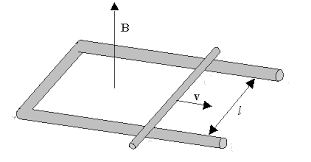
\includegraphics{Media/circuito_mobile}
	\caption{Cirucuito Mobile}
	\label{fig:circuitomobile}
\end{figure}

Si consideri ad esempio il seguente circuito mobile, avremo che una variazione del flusso genererà una $fem$ indotta, che a sua volta corrisponderà ad una corrente indotta. Come visto nella \textbf{prima legge di Laplace} sappiamo che ad una corrente corrisponde un \textbf{campo}, anche questo \textbf{indotto}, che si andrà ad opporre all'aumento di flusso. Per fare questo ovviamente il campo magnetico indotto sarà \textbf{antiparallelo} al campo $B$ della figura, dunque la corrente indotta scorrerà in senso \textbf{antiorario}. 

\subsection{Causa della forza elettromotrice indotta}
All'interno della barretta che scorre sul circuito mobile di Faraday, abbiamo delle \textbf{cariche libere} di muoversi. Ipotizziamo di andare a zoomare su una di queste cariche. Su di essa agisce un campo $\vec{B}$, ed è in \textbf{moto} a velocità $\vec{v}$. Per questo motivo ad ogni carica libera corrisponderà una \textbf{forza di Lorentz} $F = qv \times B$. Essendo libere di muoversi le cariche all'interno di questa barretta avremo una \textit{separazione} tra cariche positive e negative (la forza viene sentita da entrambe in uguale direzione e verso, le cariche negative ribaltano il verso della forza). Ad una tale separazione di cariche, corrisponde un campo dalle cariche positive a quelle negative, e conseguentemente una \textbf{differenza di potenziale} che va dalle negative alle positive. Tale differenza di potenziale è esattamente la nostra \textbf{forza elettromotrice}, che ci sarà possibile calcolare anche con questo approccio. 

Ricordando la formulazione della forza di Lorentz giungiamo al calcolo seguente: 

$$
\mathcal{E} = \left(\int F/q \cdot dl\right) = \oint v \times B = -vBl
$$

Dove il meno si riferisce ad un contesto in cui l'asse $y$ è rivolto in direzione \textit{entrante} (vedi esercizio 6).

\section{Autoinduzione - circuito RL}
Siamo in questo momento nella situazione descritta dalla figura \ref{fig:circuitomobile} e abbiamo trattato il bilancio energetico corrispondente ad un circuito minimo composto da un generatore e da una resistenza equivalente (vedi es. 6 sulle note), nel quale viene applicata una semplice legge di ohm.

$$
\mathcal{E}_{indotta} = Ri
$$

e, moltiplicando ambo i lati per un'intensità di corrente

$$ 
P_{erogata} = \mathcal{E}_{indotta}i  = P_{dissipata} = Ri^2
$$

Andiamo ora ad ampliare quanto visto fino a questo momento. Ipotizziamo che ad un certo istante $t_0$ abbiamo $v(t_0) = 0, i(t_0) = 0$, e che ad un certo punto passiamo da $i = 0$ ad una certa $i$ di \textbf{regime}. Avremo certamente un processo tramite il quale questa corrente varia per arrivare al valore di regime. Siamo interessati proprio a questo meccanismo. 

Abbiamo visto come una corrente positiva va a generare un flusso positivo (\textbf{autoflusso}) e viceversa, formalizzando questo fatto richiamando il fatto che 

$$
\Phi(B) = Li
$$

dove $L$ rappresenta l'\textbf{induttanza} ($L > 0$). 
Immaginiamo di avere un circuito dotato di un interruttore, un generatore $V_0$ e una resistenza equivalente $R$. Nel momento in cui l'interruttore viene chiuso osserveremo un'intensità di corrente, che chiaramente non sarà immediatamente l'intensità di regime, durante il periodo in cui la corrente aumenta avremo anche una \textit{variazione del flusso}, e dunque una forza \textbf{contro elettromotrice} data dalla variazione di quest'ultimo (Faraday).

In modo analogo immaginiamo di chiudere il nostro interruttore, avremo di nuovo una intensità di corrente variabile nel tempo, allo stesso modo un flusso variabile dato da $Li$ e quindi una forza \textbf{contro elettromotrice} 

$$ 
\mathcal{E}_{contro elettromotrice} = - L \frac{di}{dt}
$$

Arriviamo dunque ad una nuova \textbf{legge di Ohm} per il circuito di accensione espressa da
\begin{large}
	\begin{equation} \label{eq_Ohm_accensione}
		V_0 - L\frac{di}{dt} = Ri
	\end{equation}
\end{large}

In modo analogo, ma staccando il generatore dal circuito, avremo la legge dello spegnimento: 

\begin{large}
	\begin{equation} \label{eq_Ohm_spegnimento}
		-L\frac{di}{dt} = Ri
	\end{equation}
\end{large}

Sarà quindi necessario aggiornare gli schemi dei nostri circuiti aggiungendo il simbolo dell'\textbf{induttanza} e una \textbf{corrente variabile nel tempo} a tutta la nostra trattazione. Si noti come a crescere e decrescere in maniera esponenziale nel caso dello \textit{spegnimento} è la \textbf{corrente}, mentre nell'\textit{accensione} a decrescere in modo esponenziale è la \textbf{corrente che manca per arrivare a regime}.

\begin{large}
	\begin{equation}
		i(t) = i_{regime}e^{-\frac{t}{\tau}}
	\end{equation}
\end{large}

dove $\tau = L/R$

\subsection{Leggi di Accensione e Spegnimento del Circuito RL}

\paragraph{Accensione} La corrente sarà data dall'intensità di regime ($V_0/R$)a cui si vuole arrivare moltiplicata per la parte esponenziale: 

$$
i(t) = \frac{V_0}{R}\left(1 - e^{-t/\tau}\right)
$$

\paragraph{Spegnimento} La corrente sarà data dalla corrente di regime che però scende in modo esponenziale: 

$$
i(t) = \frac{V_0}{R} e^{-t/\tau}
$$

Si noti come siamo in presenza di \textbf{circuiti non lineari}.

\subsection{Bilancio Energetico}
Andiamo ora a vedere di ritoccare il bilancio energetico guardando cosa succede in un circuito RL che viene modificato dalla presenza dell'\textbf{induttanza}. 
Vogliamo andare a vedere quale è il lavoro esterno necessario all'accensione della corrente. In particolare avremo che per andare $i=0$ a una certa $i_{regime}$ facciamo lavoro \textbf{contro l'autoinduzione}, e questo lavoro si trova immagazzinato come \textbf{energia della corrente} (del sistema). Sarà necessario che dall'esterno sia fornita una \textbf{potenza esterna} $-\mathcal{E}_L i$.

\begin{large}
	\begin{equation}
		L = \int\left(Li\frac{di}{dt}\right) dt = \frac{1}{2} Li^2
	\end{equation}
\end{large}

Questa equazione fornisce l'\textbf{energia intrinseca della corrente} che è una quantità reversibile (accensione e spegnimento).

\section{Energia di un Sistema di Correnti}
Immaginiamo di avere un sistema inizialmente composto soltanto da un circuito composto da $i_1$, per costruire tale primo circuito compiamo un lavoro pari ad $\frac{1}{2}Li_1^2$, dobbiamo in pratica fare lavoro soltanto contro l'autoinduzione. 

Ipotizziamo ora di mettere un altro circuito percorso da corrente $i_2$.

Abbiamo visto che esiste un \textbf{coefficiente di mutua induzione}, grazie alla quale sappiamo che $\Phi_{1\rightarrow2} = Mi_1$ e che, analogamente $\Phi_{2\rightarrow1} = Mi_2$. Nel momento in cui facciamo variare la $i_1$ nel tempo, varierà anche il flusso, e dunque per Faraday osserveremo $\mathcal{E}_{indotta}$.

Tornando dunque alla nostra situazione iniziale, nel momento in cui facciamo variare $i_2$ avremo, oltre al lavoro contro l'autoinduzione, un \textbf{flusso mutuo} su i due circuiti, dunque nel momento in cui il nostro sistema è composto dai due circuiti, il lavoro esterno sarà dato da $1/2 Li_1^2 + 1/2Li_2^2 + Mi_1i_2$. Questo perché nel momento in cui accendiamo $i_2(t)$ avremo $\mathcal{E}_{2\rightarrow1} = -M\frac{di_2}{dt}$ dunque il lavoro esterno espresso in \textit{potenza} sarà dato da $-\mathcal{E}_{21}i_1$ e integrando tale potenza nel tempo, otterremo il lavoro: 

$$
L_{est} = \int Mi_1\frac{di_2}{dt}dt = Mi_1i_2
$$

Andando a generalizzare ad $n$ circuiti otteniamo la seguente formula per l'energia: 

\begin{large}
	\begin{equation} \label{eq_energia_n_circuiti_RL}
		\mathcal{U} = \sum_{k=1}^{n} \frac{1}{2} Li_k^2  + \frac{1}{2} \sum_{k,l k\ne l}^n M i_k i_l
	\end{equation}
\end{large}

L'importante quindi sarà sempre ricordare che nel momento in cui andiamo a costruire un sistema di n circuiti il lavoro esterno per costruire tale sistema è necessario considerare l'\textbf{energia intrinseca} della corrente oltre a quella di \textbf{interazione} trai due circuiti. 


\section{Equazioni di Maxwell}
Vediamo intanto le equazioni nel caso \textbf{stazionario}: 
\bigskip

\begin{center}
\begin{large}
	\begin{tabular}{|c|c|}
		\hline
		$\oint_{\Gamma} \vec{E} \cdot dl = 0 $	& Campo Elettrostatico \textbf{conservativo} \\	
		\hline
		$\oint_{sup} \vec{E} \cdot \hat{n} dS$ & Teorema di \textbf{Gauss} \\
		\hline
		$\oint_{\Gamma} \vec{B} \cdot dl = \mu_0 i$ & Teorema di \textbf{Ampere} \\ 
		\hline
		$\oint_{sup} \vec{B} \cdot \hat{n}dS = 0$ &   Flusso di B \textbf{nullo} \\
		\hline
	\end{tabular}
\end{large}

\end{center}

\bigskip

Passiamo ora al caso \textbf{non stazionario}, ovvero introducendo il \textbf{tempo} alla trattazione

\bigskip

\begin{center}
	\begin{large}
		\begin{tabular}{|c|c|}
			\hline
			$\oint_{\Gamma} \vec{E} \cdot dl = -\frac{d\Phi(B)}{dt} $	& Teorema di \textbf{Faraday}\\	
			\hline
			$\oint_{sup} \vec{E} \cdot \hat{n} dS$ & Teorema di \textbf{Gauss} \\
			\hline
			$\oint_{\Gamma} \vec{B} \cdot dl = \mu_0 i + \mu_0\epsilon_0 \frac{d\Phi(E)}{dt}$ & Introdotta Corrente di Spostamento \\ 
			\hline
			$\oint_{sup} \vec{B} \cdot \hat{n}dS = 0$ &   Flusso di B \textbf{nullo} \\
			\hline
		\end{tabular}
	\end{large}
\end{center}

Notiamo che nel caso stazionario campo elettrico e campo magnetico sono \textbf{disaccoppiati} mentre nel caso non stazionario abbiamo che la \textbf{variazione di flusso dell'uno genera l'altro}.
